\documentclass[journal,transmag]{IEEEtran}


\usepackage[noadjust]{cite}
\usepackage{physics}
\usepackage{mathtools}
\usepackage{amsmath}
\usepackage{bm}
\usepackage{calc}
\usepackage{listings}
\usepackage{url}
\usepackage{rotating}
\usepackage{calrsfs}
\usepackage{amsfonts}
\usepackage{pgf,tikz}
\usepackage{mathrsfs}
\usetikzlibrary{arrows}
\usepackage{subfig}
\usepackage{gensymb}
\hyphenation{}

\newcommand{\dimensional}[1] {
 \left[\vb{#1}\right]
 }

\lstdefinestyle{customc}{
  belowcaptionskip=1\baselineskip,
  breaklines=true,
  frame=L,
  xleftmargin=\parindent,
  language=C,
  showstringspaces=false,
  basicstyle=\footnotesize\ttfamily,
  keywordstyle=\bfseries\color{green!40!black},
  commentstyle=\itshape\color{purple!40!black},
  identifierstyle=\color{blue},
  stringstyle=\color{orange},
}

\lstdefinestyle{codeStyleC}{
language=C++,
basicstyle=\ttfamily\small,
keywordstyle=\color{blue}\ttfamily,
stringstyle=\color{red}\ttfamily,
commentstyle=\color{green}\ttfamily,
breaklines=true,
columns=flexible,
gobble=4,
xleftmargin=\leftmargini,
frame=L,
numbers=left,
numberstyle=\tiny,
belowcaptionskip=0.5em,
belowskip=1em,
}

\lstdefinestyle{codeStyleCUDA}{
language=C++,
basicstyle=\ttfamily\small,
keywordstyle=\color{blue}\ttfamily,
keywordstyle=[2]\color{darkgreen},
keywordstyle=[3]\color{red},
stringstyle=\color{red}\ttfamily,
commentstyle=\color{green}\ttfamily,
breaklines=true,
columns=flexible,
gobble=4,
xleftmargin=\leftmargini,
frame=L,
numbers=left,
numberstyle=\tiny,
keywords=[2]{__global__,__host__,__device__,__synchThreads()},
keywords=[3]{atomicAdd},
belowcaptionskip=1em,
belowskip=1em,
}

\lstdefinestyle{codeStyleFORTRAN}{
language=FORTRAN,
basicstyle=\ttfamily\small,
keywordstyle=\color{blue}\ttfamily,
keywordstyle=[2]\color{darkgreen},
stringstyle=\color{red}\ttfamily,
commentstyle=\color{green}\ttfamily,
breaklines=true,
columns=flexible,
gobble=4,
xleftmargin=\leftmargini,
frame=L,
numbers=left,
numberstyle=\tiny,
keywords=[2]{__global__,__host__,__device__,__synchThreads()},
belowcaptionskip=2em,
belowskip=5em,
}

\begin{document}


\title{A GPU Accelerated Multi-Agent Based Bird Flocking model}


%----AUTHORS------------------------------------------------------------------------------------------------------------------------
% author names and affiliations
% transmag papers use the long conference author name format.

% 		\author{\IEEEauthorblockN{Rahmat Hidayat\IEEEauthorrefmark{1,2},
% 		Davide Spataro\IEEEauthorrefmark{2},
% 		William Spataro\IEEEauthorrefmark{2},
% 		Donato D'Ambrosio\IEEEauthorrefmark{2}}
% 		
% 		\IEEEauthorblockA{\IEEEauthorrefmark{1}University Of Calabria,
% 		Department of Mathematics and Computer Science, Italy}
% 		\IEEEauthorblockA{\IEEEauthorrefmark{2}IT Division BPJS Kesehatan, Indonesia}
% 		}

%\thanks{Manuscript received December 1, 2012; revised September 17, 2014.
%Corresponding author: M. Shell (email:
% http://www.michaelshell.org/contact.html).}}



%




\IEEEtitleabstractindextext{%
\begin{abstract}
Birds flocking is an interesting natural phenomenon to study as proven by
numerous papers in this field. In this paper, we present a massive birds
flocking simulation using the GPGPU CUDA framework. This technology has been
widely adopted in computational science fields and dramatically increase
computation performances. Using the autonomous agent approach with multi-agents
and multiple groups for birds flocking modeling, we present both aggregate
motion of a large number of birds in virtual environment and other species or
predators avoidance in the plane as well. From  these experiments we gained
significant performance improvements in the terms of speedup. In
conclusion, the work shows that the use of  the CUDA technology can be effective
to cut computational costs also in multi agent modeling.
\end{abstract}

% Note that keywords are not normally used for peerreview papers.
\begin{IEEEkeywords}
GPGPU, CUDA, flocking, modelling, agents
\end{IEEEkeywords}}




\maketitle



\IEEEdisplaynontitleabstractindextext



\IEEEpeerreviewmaketitle







\chapter{Introduction}


Over the last two decades, a lot has changed regarding the way modern scientific applications are designed, written and executed, especially in the field of data-analytics, scientific computing and visualization. The main reasons behind these changes are that the size of the problems that scientists try to tackle nowadays is much bigger and because of the amount of available raw data that can be analyzed has widened the spectrum of computing applications. Data analytics and big-data techniques are applied in pretty much every field of science and have been exploited effectively also by governments and corporate organizations.

Traditionally, performance improvements in computer architecture have come from cramming more functional units onto silicon, increasing clock speeds and transistors number. Coupled with increasing clock speeds, CPU performance has until recently doubled every two years.  But it is important to acknowledge that this trend cannot be sustained indefinitely or forever. Increased clock speed and transistor number require more power and consequently generate more heat, at the point that the heat emitted from the modern processor, measured in power density rivals, the heat emitted by a nuclear reactor core!
But the power demand did not stop in over the years and is not going to stop in the near future,  and from these reasons comes the necessity of relying heavily on parallel architectures. Multi-core CPUs ($2$,$4$,$8$,$12$, up to $40$)  are ubiquitous at the point that even smart-phones are proper multi-core machines. Dedicated computing machines are nowadays large, powerful agglomerates of multi-core computing nodes interconnected via  network. Those kind of parallel machines are complex and their efficient programming is hard, bug-prone and time-consuming. 

In the field of scientific computing, and of modeling and simulation especially, parallel machines are used to obtain an approximate numerical solution to differential equations which describe physical system rigorously, as for example for the \textit{Maxwell's} equations at the foundation of classical electromagnetism or the \textit{Navier-Stokes} for fluid dynamics.
The classical approach, based on calculus, often fails to solve these kinds of equations analytically, making a numerical computer-based approach absolutely necessary.
Approximate numerical solution of partial differential equation can be obtained by applying a number of methods, as the finite element or finite difference method which yields approximate values of the unknowns at a discrete number of points over the domain.
When large domains are considered, large parallel machines are required in order to process the resulting huge amount of mesh nodes. Parallel programming is notoriously complex often requiring great programming efforts in order to obtain efficient solvers targeting large computing cluster. This is especially true since heterogeneous hardware and GPGPU has become mainstream.

The main thrust of this work is the creation of a programming abstraction and a runtime library for seamless implementation of numerical methods on regular grids targeting different computer architecture: from commodity single-core laptops to large clusters of heterogeneous accelerators. A framework, \texttt{OpenCAL} had been developed, which exposes a domain specific language for the definition of a large class of numerical models and their subsequent deployment on the targeted machines. Architecture programming details are abstracted from the programmer that with little or no intervention at all can obtain a \textit{serial, multi-core, single-GPU, multi-GPUs and cluster of GPUs} \texttt{OpenCAL} application. 
Results show that the framework is effective in reducing programmer effort in producing efficient parallel numerical solvers.

The rest of the document is organized as follows:
Chapters \ref{ch:FDM} and \ref{ch:parallel_computing} introduce the main targeted numerical models and parallel architectures, respectively.
Chapters \ref{ch:opencal}  describes \texttt{OpenCAL}, its implementation and different versions, usage and performance on a number of benchmarks, while Chapter \ref{ch:opencal_cluster} introduces the multi-GPU and distributed memory version of \texttt{OpenCAL} and evaluates its performance on three  kinds of applications, each with different computational and memory requirements.
Eventually, Chapters \ref{ch:bacteria} and  \ref{ch:flocking} introduce other HPC numerical modeling and simulation applications that have been investigated. 
In particular, Chapter \ref{ch:bacteria} introduces a specialized framework based on \texttt{OpenCAL} for tracking particle-like objects from a time-lapse video which has been applied to analyze the motility  the of \textit{B. subtilis} bacterium, while Chapter \ref{ch:flocking} investigates multi-agent collective system acceleration on GPU.
Appendix \ref{ch:stream_compaction} refers to an ad-hoc stream-compaction algorithm specifically targeting NVIDIA newest hardware that was investigated during the work on \texttt{OpenCAL}.

\section{The ACIADDRI Model}
\label{sect:aciaddri}

This work is  based on flocking behavior that was proposed by Craig W. Reynolds
in 1987 and extends it by adding the support to coexistence and interaction
between different species and predator avoidance.
Reynolds was amongst the first to abstract this behaviour to steer a swarm
of simulated birds which he called boids\cite{Reynolds}(contraction of birdoid).
Every boid has some limitations:
it has a strictly local knowledge of the space it occupies and its knowledge
comes from a simulated vision from its current position, in other words there is
no centralized control. The flock takes its decisions in a totally distributed
manner in order to obtaining a synchronized movement. More specifically, he
considered three behavioural rules each bird obeys:

\begin{description}
\item[\textsc{Cohesion}] \hfill\\
	to attempt to stay close to nearby flockmates
\item[\textsc{Collision Avoidance/Separation}] \hfill\\
	to evade obstacles and flock mates which are too
close
\item[\textsc{Velocity/Heading matching}] \hfill\\
	also called \textit{alignment}, to move in the same direction as nearby flock
	mates.
\end{description}

The \textsc{Aciaddri} model describes the environment and each bird's specie  by
means of  sets of parameters as follows:


\subsection{Environment Parameter}
 The environment is described by means of its width, length, height and by the
 time step parameter i.e. the duration in seconds of a single computational
 step. 
 \begin{table}[h!]
	\centering
	\begin{tabular}{l l l l}
	\hline
	Name & Symbol & Dimension & Description\\
	\hline
	Length &  \(W_x\) & $\dimensional{L}$ & Length of the environment \\
	Height & \(W_y\) & $\dimensional{L}$ & Height of the environment \\
	Width & \(W_z\) & $\dimensional{L}$ & Width of the environment \\
	Time Step & \(t\) & $\dimensional{T}$ & computational step duration \\
	\hline
	\end{tabular}
	\caption[List of Environment Parameters]{List of Environment Parameters of Birds Flocking}
	\label{tab:EnvironmentParameters}
\end{table}


\(W_x\), \(W_y\), and \(W_z\) are the dimension of the environment that represent 1 pixel as 1 meter. \(t\) is computational duration where 1 time step equivalent to 1 processing time.

\subsection{Species Parameters}
Each specie is described by a set of parameter that represent quantities that
are involved in the flight and flocking dynamics.

\begin{table*}
\centering
	\begin{tabular}{|l | l| l| l|}
	\hline
	Name & Symbol & Dimension & Description\\
	\hline
	Size & $s$ & $\dimensional{L}$ & Size of the bird \\
	Peak Velocity & \(v_p\)  & $\dimensional{L}\dimensional{T^{-1}}$  & The maximum velocity\\
	Thrust 	& \(a\) & $\dimensional{L}\dimensional{T^{-2}}$  & The maximum acceleration\\
	Horizontal Range of View & \(s_h\) & \(-\) & Maximum horizontal range of view\\ 
	Vertical Range of View & \(s_v\) 	& \(-\) & Maximum vertical range of view\\
	Sight Distance & \(d_s\) & $\dimensional{L}$ & Maximum sight distance\\
	Minimum Distance & \(d_{min}\) & $\dimensional{L}$  & The minimum distance between two birds to avoid collision\\
	Alignment Radius & \(d_a\) & $\dimensional{L}$  & The maximum distance bird consider to align\\
	Other Species Avoidance Radius & \(r_s\) & $\dimensional{L}$ & The minimum distance bird avoid other species\\
	Predator Avoidance Radius & \(r_p\) & $\dimensional{L}$ & The minimum distance bird avoid predator\\
	Maximum Polar & \(\theta_{max}\) & \( \dimensional{rad}\dimensional{T^{-1}} \)
	& Maximum Polar turn angle per time step\\
	Maximum Azimuthal & \(\phi_{max}\) & \( \dimensional{rad}\dimensional{T^{-1}}\) & Maximum azimuthal tung angle per time step
	\\ Wander Distance & \(w_d\) &
	\( \dimensional{L} \)& The maximum wandering distance\\
	Wander Radius & \(w_r\)	& \( \dimensional{rad}\dimensional{T^{-1}} \) & The maximum radius wandering from the target\\
	\hline
	\end{tabular}
	\hfill \\
	\caption[List of Bird Parameters]{List of Bird Parameters with values considered for the simulation}
	\label{tab:BirdParameters}
\end{table*}

The  bird's wingspan \(s\) is used as an approximation of the volume
it occupies. \(v_p\) is the maximum velocity it can travel and \(a\) represents bird's maximum acceleration.
Each bird has a limited sight of view that is described by its maximum
horizontal, \(s_h\), and vertical, \(s_v\) field of view (see images
\ref{fig:hFOV} and \ref{fig:vFOV}) and by \(d_s\) that is the maximum sight
distance of bird i.e. the maximum distance at which the bird can observs
objects.
Vertical and horizontal FOV together with the maximum sight distance define the
viewing frustum. Table \ref{tab:BirdParameters} shows the complete list of the used
parameters and corresponding alongside.


\begin{figure}
		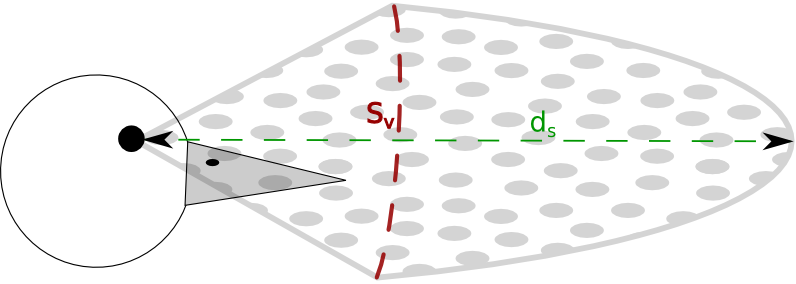
\includegraphics[scale=0.45]{./images/verticalFow.png}
		\label{fig:vFOV}
		\caption{Birds vertical field of view.}
\end{figure}	
	
	
\begin{figure}[b]
\centering
	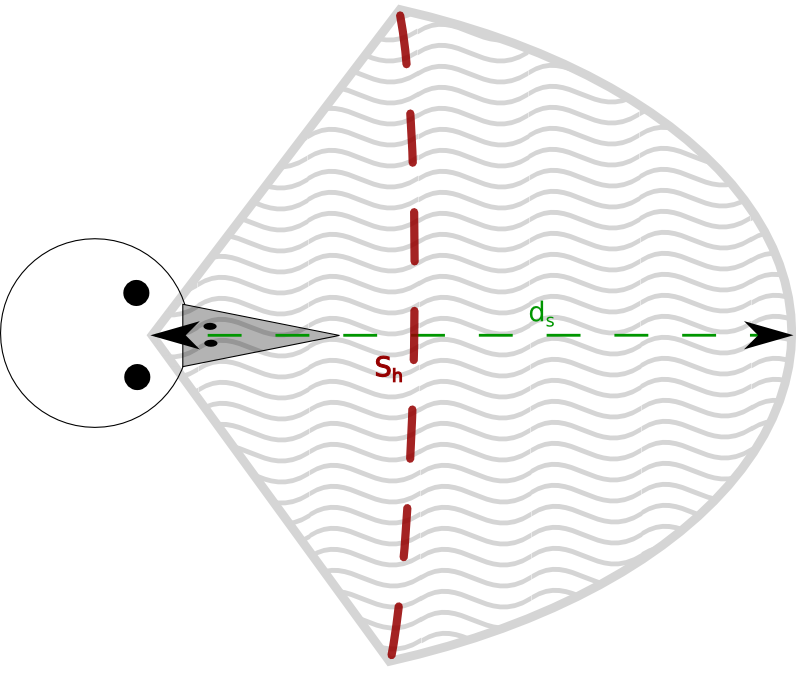
\includegraphics[scale=0.375]{./images/hFow.png}
	\label{fig:hFOV}
	\caption{Birds horizontal field of view.}
\end{figure}	
	




\subsection{Flight Model}
Bird $b$ flight at step $i$ is described by its $3$-dimensional space vectors
position $\vec{p}_b^i=\expval{p^i_x,p^i_y,p^i_z}$ and velocity
$\vec{v}_b^i=\expval{v^i_x,v^i_y,v^i_z}$, that correspond to its current sight
direction. 


The evolution of the bird's  velocity over time is regulated by
the following:

\begin{align}
\label{eq:birdCumulativeVelocities}
\vec{v}_b^{i+1} = (r \sin \theta' \cos \phi',r \sin \theta' \sin \phi',r
\cos\theta')
\end{align}




where:
\begin{itemize}
  \item $
     \theta' = \begin{cases}
    \theta_d &\mbox{ if }  |\theta_b - \theta_d| < \theta_{max}\\
    \theta_b + \theta_{max} &\mbox{ otherwise }\\
    \end{cases}
  $ \hfill \\
  
    \item $
     \phi' = \begin{cases}
    \phi_d &\mbox{ if }  |\phi_b - \phi_d| < \phi_{max}\\
    \phi_b + \phi_{max} &\mbox{ otherwise va aggiustato il segno a seconda se
    bisogna andare a destra o sinistra}\\
    \end{cases}
  $ \hfill \\ 
   

\item $ \vec{v}_d^i = \mu_c \vec{v}_c + \mu_s\vec{v}_s + \mu_a \vec{v}_a + \mu_{a} \left(
\vec{{\tau}_i} + \vec{\Gamma}_i \right) + \vec{\omega}_i $

\begin{itemize}
	\item $\mu_c$, $\mu_s$, $\mu_a$ are the cohesion, separation and alignment coefficient (social coefficients) and $\mu_a$ is the avoidance coefficient. 
\end{itemize}
\item  $\vec{v}^i_c$,$\vec{v}^i_s$, $\vec{v}^i_a$ are the  \textit{social velocities} \cite{Hemelrijk}
  \begin{itemize}
    \item $\vec{v}^i_c$, the cohesion velocity that has direction parallel to the
    line that pass through $\vec{p}_b^i$ and the average position of its neighbors
    \item $\vec{v}^i_s$, the separation velocity, keep the bird at a minimum
    safety distance from its flockmates
    \item  $\vec{v}^i_c$, the align velocity, synchronize boids heading
  \end{itemize}
 \item $\theta_d,\theta_b$ are the polar angle of the velocity vector
 $\vec{v}^i_b$ and $\vec{v}^i_d$ respetively
 \item $\phi_d,\phi_b$ are the azimuthal angle of the velocity vector
 $\vec{v}^i_b$ and $\vec{v}^i_d$ respetively


\end{itemize}


\subsection{Bird's Field of View}
Each bird has a limited visual capacity described by its field of view (FOV).
This implies that it can only perceive objects that are within its FOV. Bird
$o$'s FOV $\mathcal{F}_p$, is here defined as the set of points $p_n$ that
satisfy equations \ref{eq:fov1},\ref{eq:fov2} and \ref{eq:fov3}. In order an
object  $n$ to be within the  observer $o$'s neighborhood, it must fall within
its viewing frustum i.e. the polar and azimuthal angle between observer's view
direction and the object are less or equal than $s_h$ and $s_v$ respectively
and the distance between them should be less than the maximum sight distance of the
observer $s_d$.
Let $\vb{p'_n}=\expval{p^x_n-v^x_o,p^y_n-v^y_o,p^z_n-v^z_o}$ the position vector of the object $n$ in the $o$'s frame of reference then $n$ is $o$'s neighbor if and only if the followings hold:
\begin{equation}
\label{eq:fov1}
	\delta_s = || \vb{p_o} - \vb{p_n} ||,\; \delta_s \leq d_s 
\end{equation}
 
\begin{equation}
\label{eq:fov2}
	\frac{-s_h}{2} \leq \theta \leq \frac{+s_h}{2}
\end{equation}

\begin{equation}
\label{eq:fov3}
\frac{-s_v}{2} \leq \phi \leq \frac{+s_v}{2}
\end{equation}
where: 
\begin{align*}
 &\phi = \arccos
	\left(\frac{p'^z_n}{\sqrt{(p'^x_n)^2 + (p'^y_n)^2 + (p'^z_n)^2}}\right) \\
	&\theta = atan2 \left(\frac{p'^y_n}{p'^x_n} \right) 
\end{align*}
See appendix \ref{app:cartToSpherical} for precide definition of $atan2$
and further details.
	
	
% 	\begin{align}
% 		\label{eq:fov1}
% 		&\delta_p = |\vec{p}_{n} - \vec{p}_{o}|,\;\; \delta_p \leq d_s \\
% 		&\Delta_\alpha = \left|\frac{\alpha - \alpha'}{2}\right|,\;\; 0 \leq
% 		\Delta_\alpha \leq s_h\label{eq:fov2} \\
% 		&\Delta_\beta = \left|\frac{\beta - \beta'}{2}\right|,\;\; 0 \leq \Delta_\beta
% 		\leq s_v \label{eq:fov3}
% 	\end{align}
% where
% $\vb{p_r}=\expval{x',y',z'} = \vec{p}_{n} - \vec{p}_{o}$,
% $\vb{p_o}=\expval{x,y,z}$,
% $\alpha = arctan \left[\frac{y}{x}\right]$,
% $\beta =arctan \left[\frac{z}{\sqrt{x^2 + y^2}}\right]$,
% $\alpha' = arctan\left[\frac{y'}{x'}\right]$,
% $\beta' = arctan \left[\frac{z'}{\sqrt{x'^2 + y'^2}}\right]$.



\subsection{Cohesion}
Cohesion is a flight behavior that attracts a bird to centroid of  its perceived
neighborhood. 
In formal terms \(\vec{C}_b^i\), the bird b's centroid at time $i$, is given by:

\begin{align}
 \vec{C}_b^i = \frac{1}{|\mathcal{N}_b|}\sum_{n=1}^{|\mathcal{N}_b|}{\vec{p}_n  \frac{d_{i,j}}{d_s}}
\end{align}

where:

\begin{enumerate}
\item \(\mathcal{N}_b\) the set of birds in b's FOV.
\item \(\vec{p}_n\) is the position of $n \in \mathcal{N}_b$
\item \(d_{i,j}\) is the distance between bird \emph{b} and its neighbor
	\emph{c}

\end{enumerate}

The $b$'s cohesion vector \(\vec{v}_c\) is then defined as follows.

\begin{equation}
\vec{v}_c^i =
	\begin{cases}
	 \frac{\vec{C}_b^i - \vec{p}_b}{|| \vec{C}_b^i - \vec{p}_b ||} +
		a, &\mbox{ if } 0 < |\vec{v}_d| \leq v_p \\
		v_p, &\mbox{ otherwise } 
	\end{cases}
\end{equation}

\subsection{Separation}
\label{sect:separation}
A bird try to keep certain distance between itself and
its neighbors. Bird $b$'s separation velocity $\vec{S}_b^i$ at time $i$ is given
by:


\begin{equation}
\vec{S}_b^i = 
	\begin{cases}
	 \left[\sum_{j \in \mathcal{N}_b}{\frac{\vec{p}_b -
\vec{p}_j}{||\vec{p}_b - \vec{p}_j||}} \;f_s\right] + a ,&\mbox{if } 0 < |\vec{S}_i|
\leq v_p\\
		v_p, &\mbox{ otherwise } 
	\end{cases}
\end{equation}



where:

\begin{enumerate}
\item \(\mathcal{N}_b\) is the number of neighbors
\item $
	f_s = \begin{cases}
	0 &\mbox{ if }  d_{i,j} > d_{min}\\
	1 - \frac{d_{i,j}}{d_{min}} &\mbox{ otherwise}
	\end{cases}$
\end{enumerate}

\subsection{Alignment}
A bird tries to match its velocity (speed and heading) with those of
nearby flockmates, a behavior called velocity alignment. Real life birds only consider a relatively small number flockmates while performing this behavior and it usually is about seven neighbors\cite{Hemelrijk}.
In formal terms, bird $b$'s alignment \(\vec{A}_b^i\) is here defined as (equation \ref{eq:alignment})

\begin{align}
  \vec{A}_i = \left[\sum_{j \in \mathcal{N}'_b}{\vec{v_j}}\;f_a\right] + a, \;\;0 < |\vec{A}_i| \leq v_p
  \label{eq:alignment}
\end{align}

where:

\begin{enumerate}
\item \(\mathcal{N}'_b \subseteq \mathcal{N}_b\) is the set of birds considered by $b$ for the alignment (e.g. the nearests).
\item \(\vec{v}_j\) is the $j$'s velocity.
\item \(f_a\) is the alignment coefficient. Let \(d_{i,j}\) the distance between bird \emph{i} and \emph{j} then \(f_a\) is given by:

\begin{equation*}
	f_a = \begin{cases}
	0 &\text{, if $ d_{i,j} > d_a$}\\
	1- \frac{d_{i,j}}{d_a} &\text{, otherwise}
	\end{cases}
\end{equation*}
\end{enumerate}

\subsection{Other species and predator avoidance}
\textsc{ACIADDRI} is a multi-agent with multiple group model where each group correspond to a different bird's specie or to the group of predators. 
Different species interaction is described in section \ref{sect:otherSpecieAvoidance} and predator avoidance in section \ref{sect:predatorAvoidance}.
\begin{enumerate}[-]
	\item \textbf{Other species avoidance}
	\label{sect:otherSpecieAvoidance}
	This behavior is similar to \textit{separation} (see section \ref{sect:separation}) with the difference that a only birds from other species are taken into consideration. In formal terms the other specie avoidance vector  \(\vec{\tau}_i\) is given by:
	
	\begin{equation}
	\vec{\tau}_i = 
		 \left[\sum_{j \in \mathcal{N}_b}{\frac{\vec{p}_b -\vec{p}_j}{||\vec{p}_b - \vec{p}_j||}} \;f_s\right] + a 
	\end{equation}
	where:
	
	\begin{enumerate}
	\item \(\mathcal{N}_b\) is the number of neighbors of specid different from the one of $b$
	\item $
		f_s = \begin{cases}
		0 &\mbox{ if }  d_{i,j} > r_s\\
		1 - \frac{d_{i,j}}{r_s} &\mbox{ otherwise}
		\end{cases}$
	\end{enumerate}
	
	
	\item \textbf{Predator avoidance}
	\label{sect:predatorAvoidance}
	The predator avoidance vector is computed by taking in consideration position and velocity (speed and heading) of all the  predators within the bird's FOV. Intuitively birds will flee from the future (step $i+1$) centroid of predators's position. Formally the predator avoidance vector $\vec{\Gamma}_b^i$ is defined as follows:
	
	\begin{align}
	\vec{\Gamma}_b^i = \left[\sum_{j \in \mathcal{P}_b }^m{\frac{\vec{p}_i -
	(\vec{p}_j+\vec{v}_j)}{||\vec{p}_i - (\vec{p}_j+\vec{v}_j)||}} \;f_{p}\right] +
	a, \;\;0 < |\vec{\Gamma}_i| \leq v_p
	\end{align}
	
	where:
	
	\begin{enumerate}
	\item \(\mathcal{P}_b\) is the $b$'s set of predators
	\item $	f_{p} = \begin{cases}
		0 &\mbox{ if }  d_{i,j} > r_p\\
		1 - \frac{d_{i,j}}{r_p} & \mbox{ otherwise}
		\end{cases}
	$ \hfill \\
	 is the predator avoidance coefficient.
	\end{enumerate}
\end{enumerate}

\subsection{Wandering}
When the neighborhood  of a bird is empty it flies pseudo-randomly in the space. This kind of behavior is called \textit{wandering}. 
Wandering is obtained combining a current and a random direction 
\begin{equation*}
    \vec{\omega}_b^i =  
		\begin{cases} 
			0 &\mbox{if } \mathbb{N} \neq \emptyset \\ 
			\frac{\vec{s}}{|\vec{s}|}\;w_r+w_d,\; 0 < |\vec{\omega}_i| \leq v_p & \mbox{otherwise }. 
		\end{cases}
\end{equation*}

\section{Parallel implementation}
\label{sect:gpuimplementation}
In this work we adopt GPUs and the CUDA framework to accelerate the flocking
simulation of a large number of boids using the the model presented in section
\ref{sect:aciaddri} in an environment with a number of agents up to $5
\times10^6$.
Seeking the APOD development methodology we produced two different parallel
versions, both sharing the high-level implementation structure that consists in
(the well-known host-managed accelerated program structure):
\begin{itemize}
	\item Initialization of data structures on \emph{CPU}
	\item Data transfer from \textbf{\emph{CPU} to \emph{GPU}}
	\item Kernels execution on \emph{GPU}
	\item Copying the result back from \textbf{\emph{GPU} to \emph{CPU}}
\end{itemize}
The parallelization strategy is designed with the purpose to avoid as much
as possible the very undesirable data copy from \emph{host to device}\cite{cita}, or vice versa.
The computation of $\vec{p}_b^{i+1}$ and $\vec{v}_b^{i+1}$ is entirerly performed on GPU and implemented as composition of CUDA kernels. Moreover Parameters are stored in constant memory for fast access.
An OpenGL 3D visualization tool comes with the simulation system and permits real time and interactive 
rendering of the flocking model.

\subsection{Na\"{i}ve version}
In this version each agent is mapped to a CUDA thread organized in a 1D block-grid structure.
All data resides in global memory and user managed cache (shared memory) remains unused. 
Due to the high parallel nature of the simulation, although its simplicity this version already yield to a speedup of $\approx20 \times$. 

\subsubsection*{If-Divergence mitigation} Thread divergence is a well known
issue, that disallow full parallelism at warp level. Two threads are said to
diverge if they belongs to the same warp but executing different
instructions\footnote{Common code constructs that usually cause thread
divergence are conditionals that depends on  thread-id variable}. If some
threads in a warp evaluate a conditional to \emph{true} and others to \emph{false}, then threads will branch to different instructions paths
and those paths are executed in \emph{serial manner}\footnote{It is important to
stress that serial execution happens only when thread of the same warp
diverge.}\cite{CUDA1}. This serialization may result in significant performance
loss.

A serie of workaraund have been implemented in order to mitigate this problem  and more specifically, a number of $if$ construct have been substituted with an equivalent arithmetical operation that are performed by all threads and preserves the original semantic of the code. Listings \ref{list:divergent} and \ref{list:notDivergent} shows an example of such translation.
\begin{lstlisting}[style=customc,caption=Thread Divergent code example, label={list:divergent}]
	private var;
	if(threadIdx.x > 16) then
		var:= A
	else
		var:= B
\end{lstlisting}

\begin{lstlisting}[style=customc, label={list:notDivergent}, caption=If mitigated version of the listing \ref{list:divergent} ]
	bool c = threadIdx.x > N
    private var;
	var:= c*A + !c*B
\end{lstlisting}


\subsection{Shared memory version}
This version exploit the shared memory in order to cache birds's frequently accessed data. Shared memory is mush faster than global memory but is of limited capacity (and depends on compute capability of the device, $48 KB$ in the \emph{GTX980}),only accessible at block level and freshed at each kernel invocation. This implies a number of restriction on its usage namely:

\begin{itemize}
	\item it has to be initializated (i.e. requires a global memory access)
    \item limited size of data available per thread
    \item 

\end{itemize}





































\section{Experimental results}
\label{sect:experiments}
In order to ensure the correctness of the parallelization the output of each
parallel version were matched against the corrensponding serial output. 



\subsection{Hardware}
\label{sec:hardware}
Three  devices were adopted for testing different CUDA version of the
model, the high-end GTX 980, Tesla K40 and a GT 635M,a low-end mobile chip(see
table \ref{tab:adoptedHW} for further details).

 \begin{table}
	\centering
	\begin{tabular}{|l |l |l| l|l|}
	\hline
	Name & Compute Capability & RAM &
	SM-Clock & \# cores\\
	\hline
	GT 653M & \(2.1\) & \(1024\)MB  & $675$ MHz  & 635\\
	GTX 980& \(5.5\) & \(4096\)MB  & $1216$ MHz & 2048 \\
	TESLA K40& \(5.2\) & \(12288\)MB  & $875$ MHz & 2880 \\
	\hline
	\end{tabular}
	\caption{Hardware utilized for experiments}
	\label{tab:adoptedHW}
\end{table}
a low end
mobile chip and a high-end GPU GT 635M, compute capability 2.1and GTX 980

\subsection{Timings}
See table \ref{tab:naive} and \ref{tab:ifdiv}.
\begin{table}
	\centering
	\begin{tabular}{|l |l |l| l|}
	\hline
	\# birds & Sequential & GTX 980 & GT
	635M
	\\
	\hline
	
	1024  & \(559.9\) & $29.1$ & $10.5$ \\
	5120  & \(920.8\) & $574.4$ & $51.7$ \\
	10240 &  $37147.9$ & 2241.6 & 109.0 \\
	15360  & \(37147.9\) & $5004.7$ & $235.2$ \\
	20480  & 148925.1 & 8868.9 & $312.5$ \\
	40960  & - & - & $1023.8$ \\
	81920  & - & - & $3663.5$ \\
	163840  & - & - & $14877.4$ \\
	327680  & - & - & $58003.0$ \\
	\hline
	\end{tabular}
	\caption{Timing (in seconds) for the Parallel CUDA Na\"ive implementation}
	\label{tab:naive}
\end{table}


\begin{table}
	\centering
	\begin{tabular}{|l |l |l| l|}
	\hline
	\# birds & Sequential & GTX 980 & GT
	635M
	\\
	\hline
	
	1024  & \(559.9\) & $19.9$ & $7.9$ \\
	5120  & \(920.8\) & $366.3$ & $34.6$ \\
	10240 &  $37147.9$ & 1398.7 & 96.5 \\
	15360  & \(37147.9\) & $3110.0$ & $154.9$ \\
	20480  & 148925.1 & 5522.0 & $280.8$ \\
	40960  & - & - & $825.4$ \\
	81920  & - & - & $3307.2$ \\
	163840  & - & - & $13565.9$ \\
	327680  & - & - & $54113.4$ \\
	\hline
	\end{tabular}
	\caption{Timing (in seconds) for the Parallel CUDA Na\"ive implementation}
	\label{tab:ifdiv}
\end{table}


\section{Conclusion}
In conclusion, the work shows that the use of the CUDA
technology can be effective to cut computational costs also in multi agent
modeling.

\subsection{Future development}
Although Reynold’s model is very good, but we also need future im-
provement in order to make simulation as well as in the real world.
Adding some parameters are needed in order to mimic how bird fly.
v s is stall velocity, in which a minimum bird’s velocity. If a bird fly
with velocity lower than its stall velocity, the bird will stall. v c is the
normal velocity of bird. Bird always tends to fly with v c when it fly in
group. Since a bird can not fly in vertical way, it is necessary to add
a parameter to represent this limitation. Θ max is the maximum angle
of bird can reach, if a bird try to fly more than this limitation, it will
stall. Wing’s length (l w ) and width (l d ) are also interesting to consider.
Different wing’s length and width will give behavior when fly.

In CUDA programming, critical process is carried out in the GPU and
then the final result is sent back to the CPU. It requires costs related to
the visualization of computational result, processing data on the GPU
and then send the results to the CPU and then visualize the result back
to the GPU is not efficient. To improve efficiency and performance, it
is necessary to implement this with OpenGL / CUDA interoperability.
Instead of sending back result to the CPU and then send back again to
GPU in order to visualize it, it is better to directly visualize the result
without passing it to the CPU is the efficient solution.







\appendices
\section{Cartesian to Spherical coordinate conversion}
\label{app:cartToSpherical}
We use the the two arguments atan version in order to to gather information on the signs of the inputs in order to return the appropriate quadrant of the computed angle, which is not possible for the singleargument arctangent function. Additionally, the ordinary arctangent  suffers when required to produce  $\pm \frac{\pi}{2} $ angle \footnote{Computing angle between $x$ and $y$ axis would require a division by zero.}.
\begin{equation*}
	\theta = 
	\begin{cases}
	
	\frac{\pi}{2},&\mbox{if }  p'^x_n=0, \ p'^y_n>0  \\
	
	\frac{3\pi}{2},&\mbox{if } p'^x_n=0, \ p'^y_n<0 \\
	
	\text{undefined} &\mbox{if } p'^x_n=0, p'^y_n =0 \\
	
	\arctan \frac{p'^y_n}{p'^x_n} &\mbox{if } p'^x_n>0, \ p'^y_n \ge 0  \\
	
	\arctan \frac{p'^y_n}{p'^x_n} + 2 \pi &\mbox{if } \ p'^x_n>0, \ p'^y_n < 0, \ \ or
	\ p'^x_n<0, \ p'^y_n > 0 \\
	
	\arctan \frac{p'^y_n}{p'^x_n} + \pi &\mbox{if }\ p'^x_n<0, \ p'^y_n \le 0 
	\end{cases}
\end{equation*}


\begin{figure}%
    \centering
    \subfloat[label 1]{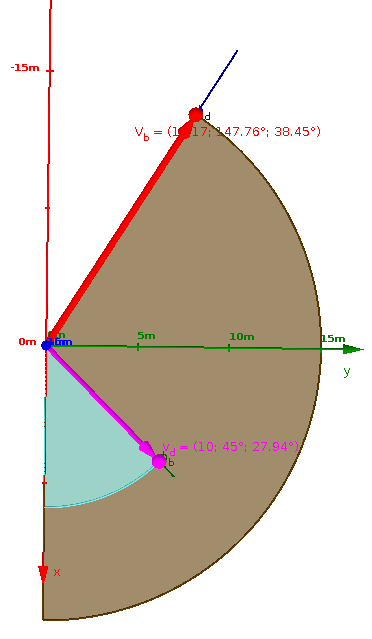
\includegraphics{./images/horizonthal.png}}%
    \qquad
    \subfloat[label 2]{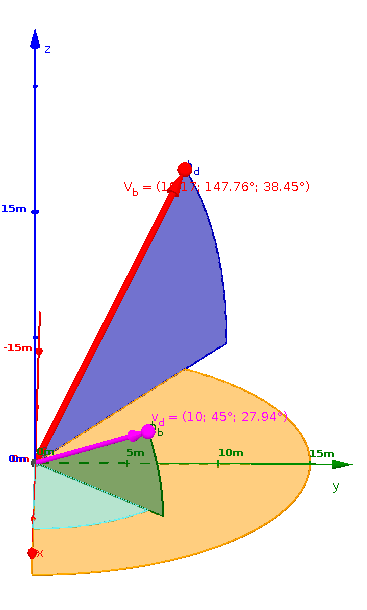
\includegraphics{./images/vertical.png}}%
    \caption{Example of spherical coordinate representation. $V_d$ for
    instance is a vector of magnitute $10$ and polar and aximuthal angles
    $45\degree$ and $27.94\degree$ respectively.}%
    \label{fig:example}%
\end{figure}

% use section* for acknowledgment
\section*{Acknowledgment}
The authors would like acknowledge, Elisa De Giorgio for pointing out the
precide formalization of  the bird's field of view and NVIDIA for providing the
GPU hardware.

\ifCLASSOPTIONcaptionsoff
\newpage
\fi



\begin{thebibliography}{1}

\bibitem{Ferber}
J. Ferber
\newblock Multi-Agent Systems: An Introduction to Distributed Artificial
Intelligence, AddisonWesley
\newblock New York, 1999

\bibitem{Woolridge}
M. Woolridge
\newblock Introduction to Multiagent Systems, John Wiley and Sons,
\newblock New York, 2001

\bibitem{Reynolds}
Reynolds, C.W.
\newblock Flocks, herds, and schools.
\newblock Computer Graphics 21(4) (1987), 25–34

\bibitem{Blumberg}
Bruce~M. Blumberg and Tinsley~A. Galyean.
\newblock Multi-level direction of autonomous creatures for real-time virtual
  environments.
\newblock {\em Computer Graphics}, 29(Annual Conference Series):47--54, 1995.

\bibitem{Cheng}
John Cheng, Max Grossman, and Ty~McKercher.
\newblock {\em Professional CUDA C Programming}.
\newblock John Wiley \& Sons, Inc, 2014.

\bibitem{Culler}
David~E. Culler, Jaswinder~Pal Singh, and Anoop Gupta.
\newblock {\em Parallel Computer Architecture, A Hardware/Software Approach}.
\newblock Morgan Kaufmann, 1997.

\bibitem{Dutta}
Kishore Dutta.
\newblock How birds fly together: The dynamics of flocking.
\newblock {\em Resonance}, 15(12):1097--1110, December 2010.

\bibitem{phys.org}
Katharine Gammon.
\newblock http://phys.org/news/2011-10-secrets-flocking-revealed.html, last
  accessed 11 september 2015, 2011.

\bibitem{Gangshan}
Gangshan Jingab, Yuanshi Zhengab, and Long Wang.
\newblock Flocking of multi-agent systems with multiple groups.
\newblock {\em International Journal of Control}, 87(12):2573–2582, July
  2014.

\bibitem{Hwu}
David~B. Kirk and Wen mei W.~Hwu.
\newblock {\em Programming Massively Parallel Processors, A Hands-onApproach}.
\newblock Morgan Kaufmann, second edition, 2013.

\bibitem{Laird}
John~E. Laird.
\newblock It knows what you're going to do: Adding anticipation to a quakebot.
\newblock {\em AAAI 2000 Spring Symposium Series: Artificial Intelligence and
  Interactive Entertainment}, pages 41--50, March 2000.

\bibitem{CUDA2}
NVIDIA.
\newblock {\em Whitepaper NVIDIA GeForce GTX 980, Featuring Maxwell, The Most
  Advanced GPU Ever Made}.
\newblock NVIDIA, 2014.

\bibitem{CUDA3}
NVIDIA.
\newblock {\em CUDA C Best Practices Guide}.
\newblock NVIDIA, 2015.

\bibitem{CUDA1}
NVIDIA.
\newblock {\em CUDA C Programming Guide}.
\newblock NVIDIA, March 2015.

\bibitem{Pacheco}
Peter~S. Pacheco.
\newblock {\em An Introduction to Parallel Programming}.
\newblock Morgan Kaufmann, 2011.

\bibitem{Reynolds3}
Craig~W. Reynolds.
\newblock Flocks, herds, and schools: A distributed behavioral model.
\newblock {\em Computer Graphics}, 21(4):25--34, 1987.

\bibitem{Reynolds2}
Craig~W. Reynolds.
\newblock Steering behaviors for autonomous characters.
\newblock {\em Game Developers Conference 1999, San Jose, California}, pages
  763--782, 1999.

\bibitem{Reynolds1}
Craig~W. Reynolds.
\newblock Interaction with groups of autonomous characters.
\newblock {\em Game Developers Conference 2000, San Francisco, California},
  pages 449--460, 2000.

\bibitem{Shiffman}
Daniel Shiffman.
\newblock {\em The Nature of Code, Simulating Natural System with Processing}.
\newblock Self Publishing, 2012.

\bibitem{Wilt}
Nicholas Wilt.
\newblock {\em The CUDA Handbook, Comprehensive Guide to GPU Programming}.
\newblock Addison-Wesley, 2013.

\bibitem{Hemelrijk}
Hemelrijk, Charlotte K. AND Hildenbrandt, Hanno (2011).
\newblock {\em Some Causes of the Variable Shape of Flocks of Birds}.
\newblock PLoS ONE 6(8), 2011.
\end{thebibliography}

% biography section
%
% If you have an EPS/PDF photo (graphicx package needed) extra braces are
% needed around the contents of the optional argument to biography to prevent
% the LaTeX parser from getting confused when it sees the complicated
% \includegraphics command within an optional argument. (You could create
% your own custom macro containing the \includegraphics command to make things
% simpler here.)
%\begin{IEEEbiography}[{\includegraphics[width=1in,height=1.25in,clip,keepaspectratio]{mshell}}]{Michael Shell}
% or if you just want to reserve a space for a photo:

% You can push biographies down or up by placing
% a \vfill before or after them. The appropriate
% use of \vfill depends on what kind of text is
% on the last page and whether or not the columns
% are being equalized.

%\vfill

% Can be used to pull up biographies so that the bottom of the last one
% is flush with the other column.
%\enlargethispage{-5in}



% that's all folks
\end{document}
